\subsubsection{Schema Speisung}
\label{sec:Schema_Speisung}

Nachfolgend wird der Speisungspfad vom USB mini-B Connector bis zu den regulierten 3.3\si{V} beschrieben.

\paragraph{USB Port}

Ein standard USB 2.0 Port kann einen maximalen Strom von ${I_{max}=500\si{mA}}$ bereitstellen.
Dieser Strom ist die obere Grenze für das DSP Board. In keinem Betriebsfall inkl. Akkuladen wird dieser maximale Strom überschritten.
\
Zum Schutz der USB-Host Geräte vor einem Kurschlussstrom, ist F1 (MF-MSMF110) mit einem Auslösestrom von ${I_{trip}=2.20\si{A}}$ \cite{usb-fuse} verbaut.


\paragraph{Battery Management (BQ2409x)}

Der BQ24093 ist ein single-cell Li-Ion / Li-Po Akkulade-IC, das speziell für USB Applikationen gemacht ist.
Die Beschaltung des \textit{IC1} ist gemäss Vorgaben aus dem Datenblatt \cite{bq2409x}.

Der Akkumulator ist nicht Teil des Systems. Aus diesem Grund ist ein 2-Pin JST-XH Connector (\textit{J6}) vorgesehen.
Weil der Akkumulator und ein entsprechender temperaturabhängiger Widerstand nicht bekannt ist, 
wird der Pin für die Temperaturüberwachung mit \textit{R19} terminiert.
\textit{IC1} wird mit dem Pull-Down \textit{R51} am \texttt{ISET2} Pin auf \texttt{LOW} gezogen, was den Ladestrom auf ${I_{charge}=100\si{mA}}$ beschränkt. 
Bei Bedarf kann der Ladestrom vom STM32 über \texttt{PB14} auf \texttt{HIGH} und damit ${I_{charge}=500\si{mA}}$ festgelegt werden.


\begin{figure} [H]
\begin{center}
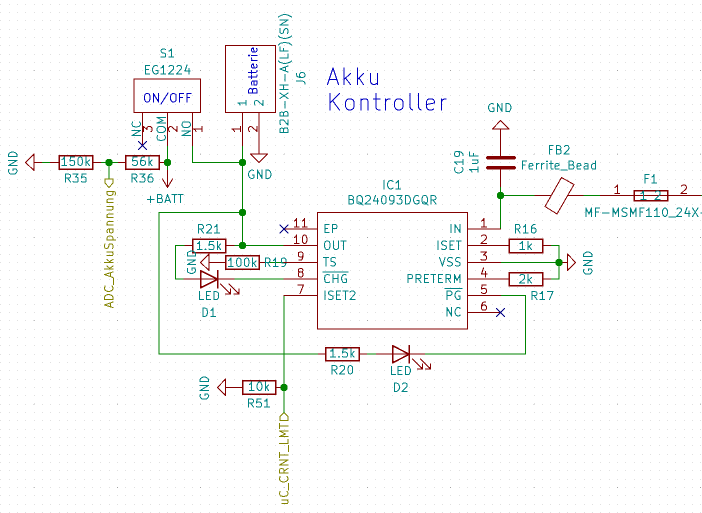
\includegraphics[scale=0.5]{../graphics/Schema_Akku.png}
\caption{BQ24093 mit äusserer Beschaltung nach Datenblatt}
\label{fig:Schema_Akku}
\end{center}
\end{figure}

\paragraph{ADC Akkumulator Spannungsmessung}

Die Akkumulatorspannung mit ${V_{bat}=4.2\si{V}}$ übersteigt den Eingangsspannungsbereich des\\
 STM32 Microcontrollers von ${V_{GPIO_{max}}=3.3\si{V}}$.
Damit zur Bestimmung des Ladestandes die Spannung gemessen werden kann, wird diese mit dem Spannungsteiler \textit{R35/R36} auf ein Maximum von 3.3\si{V} heruntergeteilt. 
Mit Widerstandswerten aus der E12-Reihe ergibt sich folgender Spannungsteiler.

\begin{equation}
V_{out_{max}} = V_{bat_{max}}*\frac{R35}{R35+R36}
\end{equation}

\begin{equation}
3.277\si{V} = 4.5\si{V}*\frac{150\si{k\Omega}}{150\si{k\Omega}+56\si{k\Omega}}
\end{equation}

Somit muss die gemessene Spannung in der Software um folgenden Faktor korrigiert werden.

\begin{equation}
F_C=\frac{V_{bat_{max}}}{V_{out_{max}}}=\frac{3.27\si{V}}{4.5\si{V}}=\underline{0.7\bar{3}}
\end{equation}

\paragraph{Energiebedarf der Schaltung}

Unten aufgeführt ist eine Abschätzung des Energiebedarfs der Schaltung, die massgebend für die Wahl der Spannungsregler ist. Die Speisung ist in analog und digital aufgeteilt.

\begin{table}[H]
\centering
\begin{tabular}{|l|r|}
\hline
\textbf{Schaltungsteil} & \textbf{$I_{max}$ {[}\si{mA}{]}} \\ \hline
STM32                   & 40                     \\ \hline
SSD1306                 & 30                     \\ \hline
SSD1306                 & 30                     \\ \hline
reserve                 & 50                     \\ \hline
\textbf{Total}          & \textbf{150}          \\ \hline
\end{tabular}
\caption{Stromverbrauch 3.3V digital}
\end{table}

\begin{table}[H]
\centering
\begin{tabular}{|l|r|}
\hline
\textbf{Schaltungsteil} & \textbf{$I_{max}$ {[}\si{mA}{]}} \\ \hline
MAX4762                 & 0.01                   \\ \hline
TLV320                  & 26.00                  \\ \hline
reserve                 & 30.00                  \\ \hline
\textbf{Total}          & \textbf{56.01}        \\ \hline
\end{tabular}
\caption{Stromverbrauch 3.3V analog}
\end{table}

Die verbauten Festspannungsregler TLC7333 \textit{(IC2, IC3)} mit Low Dropout Voltage können bis zu ${I_{out}=300\si{mA}}$ liefern.

\paragraph{Verlustleistung der Spannungsregler}

Die maximale Verlustleistung an einem der Spannungsregler \textit{(IC2, IC3)} tritt auf, wenn die Eingangsspannung ${V_{in}=5\si{V}}$ beträgt und der maximale Strom von ${I_{max}=0.15\si{A}}$ fliesst.
Dabei entsteht eine Verlustleistung von:

\begin{equation}
P_{LDO_{max}}=(5.0\si{V}-3.3\si{V})*0.15\si{A}=0.255\si{W}
\end{equation}

